\documentclass[11pt,a4paper]{article}

\usepackage[a4paper,margin=1.7cm]{geometry}
\usepackage[T1]{fontenc}
\usepackage{lmodern}
\usepackage{microtype}
\usepackage{booktabs}
\usepackage{tabularx}
\usepackage{array}
\usepackage{graphicx}
\usepackage{caption}

\pagestyle{empty}
\setlength{\parindent}{0pt}
\setlength{\parskip}{0.5em}
\captionsetup{font=small,labelfont=bf,skip=4pt}
\newcolumntype{L}{>{\raggedright\arraybackslash}X}
\newcolumntype{R}{>{\raggedleft\arraybackslash}p{1.55cm}}

\begin{document}

{\Large\bfseries Monthly temperature panel, Hong Kong Observatory Headquarters, 2013--2023}

\vspace{0.15em}
{\small Prepared 12 August 2026 by Shen Ruililin.\quad
Public climate only.\quad No Hospital Authority columns.}

\vspace{0.4em}
This note accompanies the attached CSV.
The join key is \texttt{month\_id} (\texttt{YYYY-MM}), January 2013 through December 2023 (132 months).
Station is Hong Kong Observatory Headquarters throughout.
Daily flags use HKO climatological thresholds; the monthly counts are a roll-up of those flags, not a new HKO definition.

\vspace{0.2em}
{\small\bfseries Columns}

\vspace{0.15em}
{\small
\begin{tabularx}{\textwidth}{@{}l L@{}}
\toprule
\texttt{month\_id} & Calendar month \\
\texttt{mean\_temp}, \texttt{mean\_tmin}, \texttt{mean\_tmax} & Monthly means of daily mean, minimum, and maximum temperature ($^\circ$C) \\
\texttt{hot\_nights} & Days with $T_{\min}\geq 28^\circ$C \\
\texttt{very\_hot\_days} & Days with $T_{\max}\geq 33^\circ$C \\
\texttt{extremely\_hot\_days} & Days with $T_{\max}\geq 35^\circ$C \\
\texttt{cold\_days} & Days with $T_{\min}\leq 12^\circ$C \\
\texttt{days\_in\_2d3n\_window} & Days belonging to a two consecutive very hot days with the three corresponding hot nights window \\
\texttt{station} & Always \texttt{HKO} in this file \\
\bottomrule
\end{tabularx}
}

\vspace{0.45em}
{\small\bfseries Table 1.} Monthly climate series, January 2013--December 2023 ($n=132$ months)

\vspace{0.2em}
{\small
\begin{tabularx}{\textwidth}{@{}L rrrrr@{}}
\toprule
Series & Mean & SD & Min & Max & 11-year total \\
\midrule
Mean temperature ($^\circ$C) & 24.02 & 4.68 & 15.24 & 30.27 & --- \\
Mean $T_{\min}$ ($^\circ$C) & 22.10 & 4.67 & 13.35 & 28.35 & --- \\
Mean $T_{\max}$ ($^\circ$C) & 26.66 & 4.80 & 17.68 & 33.32 & --- \\
Hot nights (days/month) & 3.40 & 5.38 & 0 & 25 & 449 \\
Very hot days (days/month) & 3.19 & 5.16 & 0 & 21 & 421 \\
Cold days (days/month) & 1.10 & 2.54 & 0 & 11 & 145 \\
Extremely hot days (days/month) & 0.31 & 1.09 & 0 & 10 & 41 \\
\bottomrule
\end{tabularx}
}

\vspace{0.35em}
Of 145 official cold days, 141 fell in December--February (December 40, January 54, February 47; March 4).
After calendar month, remaining cold-day variation is between-year differences within winter.

\vspace{0.25em}
{\small Please do not append health counts to the CSV if you circulate it.
Page 2 shows the same daily Headquarters series as annual totals, checked against HKO Year's Weather summaries.}

\clearpage

\begin{figure}[p]
\centering
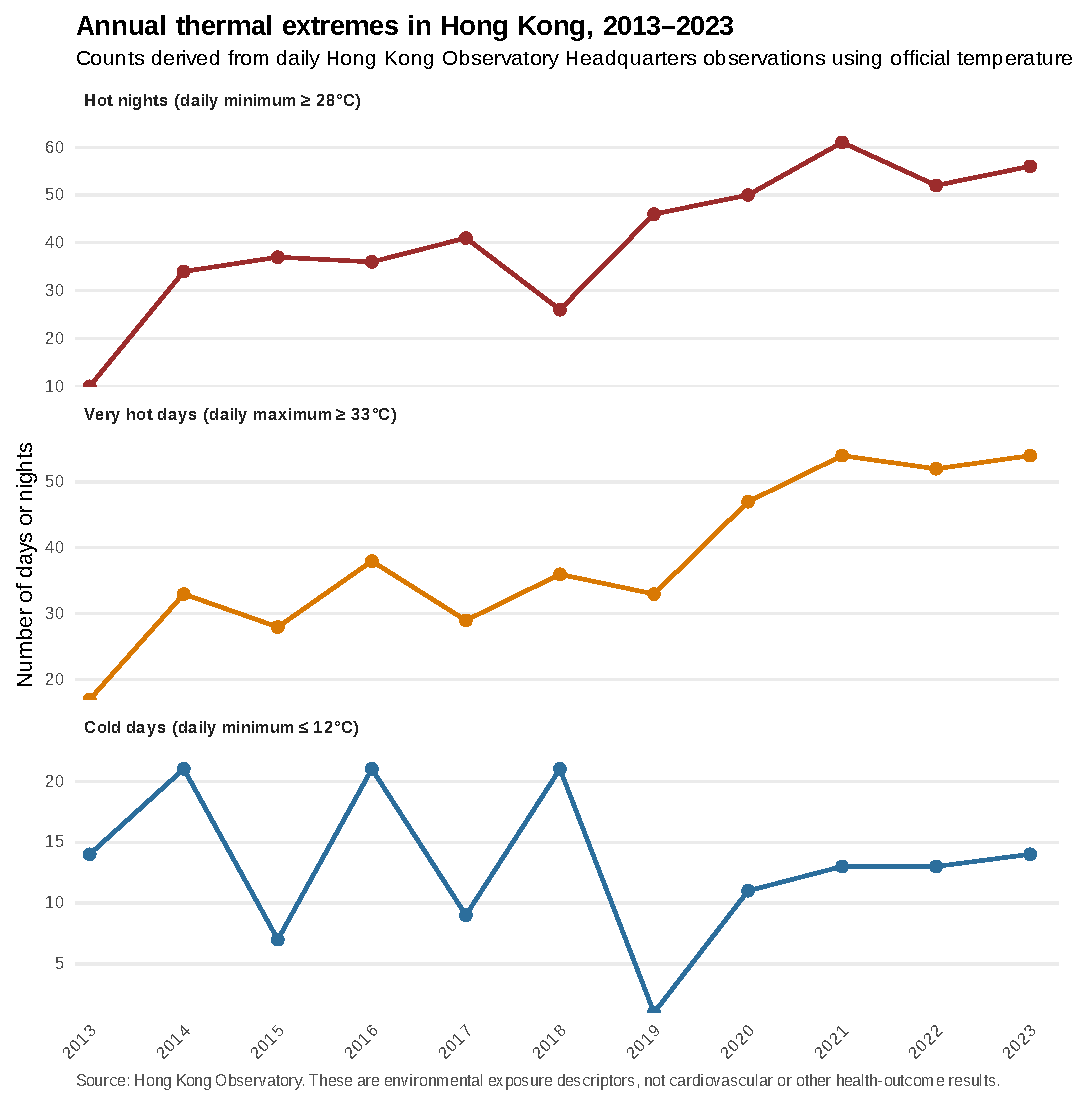
\includegraphics[width=0.92\textwidth]{../../figures/hko_annual_extremes_2013_2023.pdf}
\caption*{Annual counts from the same Headquarters daily series.
These are environmental descriptors, not hospitalisation results.}
\end{figure}

\end{document}
